\begin{center}
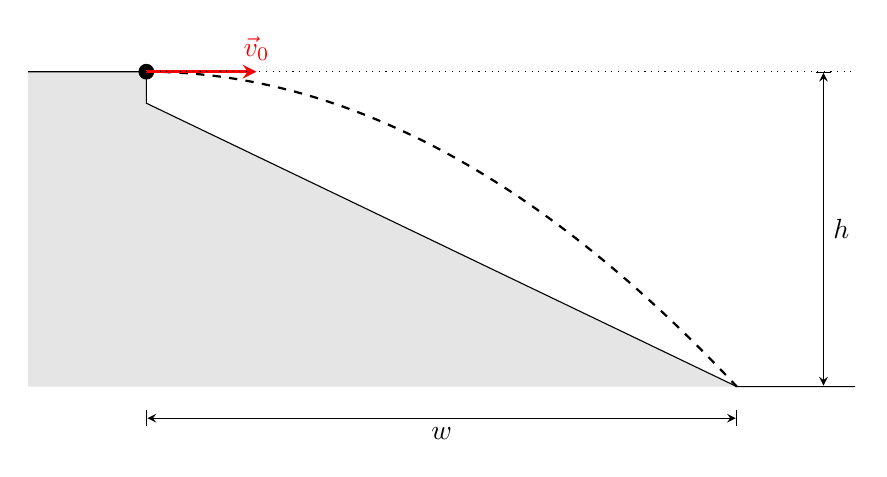
\begin{tikzpicture}[>=stealth]
 \fill[gray!20] (-1.5,0) -- (-1.5,4) -- (0,4) -- (0,3.6) -- (7.5,0) -- cycle;
 \draw (-1.5,4) -- (0,4) -- (0,3.6) -- (7.5,0) -- (9,0);
 \draw[thick, dashed, domain=0:7.5, samples=50] plot (\x, {4-4*(\x/7.5)^2});
 \fill (0,4) circle (0.1);
 \draw[->, very thick, red] (0,4) -- (1.4,4) node[above] {$\vec v_0$};
 \draw[dotted] (0,4) -- (9,4);
 \draw[|<->|] (8.6,0) -- (8.6,4) node[midway, right] {$h$};
 \draw[|<->|] (0,-0.4) -- (7.5,-0.4) node[midway, below] {$w$};
\end{tikzpicture}
\end{center}

Vertikal fällt der Springer (ohne Luftwiderstand und Auftrieb) wie beim freien Fall. Für die Höhe $h$ braucht er die Zeit
\begin{align}
 h &= \frac{1}{2}g\,t^2 \quad\Rightarrow\quad t = \tsF = \ts
\end{align}
Horizontal bewegt er sich gleichförmig mit $v_0$:
\begin{align}
 w &= v_0\,t = \xsF \\
   &= \vs\cdot\sqrt{\frac{2\cdot\hs}{\gE}} \\
   &= \xs \approx \result{\xsP{0}{2}}
\end{align}
